\documentclass{article}
\usepackage{amsfonts, amsthm, amsmath, amssymb, mathtools, ulem, mathrsfs, physics, esint, siunitx, tikz-cd}
\usepackage{pdfpages, fullpage, color, microtype, cancel, textcomp, markdown, hyperref, graphicx}
\usepackage{enumitem}
\usepackage{algorithm}
\usepackage{algpseudocode}
\graphicspath{{./images/}}
\usepackage[english]{babel}
\usepackage[autostyle, english=american]{csquotes}
\MakeOuterQuote{"}
\usepackage{xparse}
\usepackage{tikz}

\usepackage{calligra}
\DeclareMathAlphabet{\mathcalligra}{T1}{calligra}{m}{n}
\DeclareFontShape{T1}{calligra}{m}{n}{<->s*[2.2]callig15}{}
\newcommand{\script}[1]{\ensuremath{\mathcalligra{#1}}}
\newcommand{\scr}{\script r}

% fonts
\def\mbb#1{\mathbb{#1}}
\def\mfk#1{\mathfrak{#1}}
\def\mbf#1{\mathbf{#1}}
\def\tbf#1{\textbf{#1}}

% common bold letters
\def\bP{\mbb{P}}
\def\bC{\mbb{C}}
\def\bH{\mbb{H}}
\def\bI{\mbb{I}}
\def\bR{\mbb{R}}
\def\bQ{\mbb{Q}}
\def\bZ{\mbb{Z}}
\def\bN{\mbb{N}}

% brackets
\newcommand{\br}[1]{\left(#1\right)}
\newcommand{\sbr}[1]{\left[#1\right]}
\newcommand{\brc}[1]{\left\{#1\right\}}
\newcommand{\lbr}[1]{\left\langle#1\right\rangle}

% vectors
\renewcommand{\i}{\hat{\imath}}
\renewcommand{\j}{\hat{\jmath}}
\renewcommand{\k}{\hat{k}}
\newcommand{\proj}[2]{\text{proj}_{#2}\br{#1}}
\newcommand{\m}[2][b]{\begin{#1matrix}#2\end{#1matrix}}
\newcommand{\arr}[3][\sbr]{#1{\begin{array}{#2}#3\end{array}}}

% misc
\NewDocumentCommand{\seq}{O{n} O{1} O{\infty} m}{\br{#4}_{{#1}={#2}}^{#3}}
\NewDocumentCommand{\app}{O{x} O{\infty}}{\xrightarrow{#1\to#2}}
\newcommand{\sm}{\setminus}
\newcommand{\sse}{\subseteq}
\renewcommand{\ss}{\subset}
\newcommand{\vn}{\varnothing}
\newcommand{\lc}{\epsilon_{ijk}}
\newcommand{\ep}{\epsilon}
\newcommand{\vp}{\varphi}
\renewcommand{\th}{\theta}
\newcommand{\cjg}[1]{\overline{#1}}
\newcommand{\inv}{^{-1}}
\DeclareMathOperator{\im}{im}
\DeclareMathOperator{\id}{id}
\newcommand{\ans}{\tbf{Ans. }}
\newcommand{\pf}{\tbf{Pf. }}
\newcommand{\imp}{\implies}
\newcommand{\impleft}{\reflectbox{$\implies$}}
\newcommand{\ck}{\frac1{4\pi\ep_0}}
\newcommand{\ckb}{4\pi\ep_0}
\newcommand{\sto}{\longrightarrow}
\DeclareMathOperator{\cl}{cl}
\DeclareMathOperator{\intt}{int}
\DeclareMathOperator{\bd}{bd}
\DeclareMathOperator{\Span}{span}
\newcommand{\floor}[1]{\left\lfloor#1\right\rfloor}
\newcommand{\ceil}[1]{\left\lceil#1\right\rceil}
\newcommand{\fxn}[5]{#1:\begin{array}{rcl}#2&\longrightarrow & #3\\[-0.5mm]#4&\longmapsto &#5\end{array}}
\newcommand{\sep}[1][.5cm]{\vspace{#1}}
\DeclareMathOperator{\card}{card}
\renewcommand{\ip}[2]{\lbr{#1,#2}}
\renewcommand{\bar}{\overline}
\DeclareMathOperator{\cis}{cis}
\DeclareMathOperator{\Arg}{Arg}

% title
\title{Scientific Computing HW 9}
\author{Ryan Chen}
%\date{\today}
\setlength{\parindent}{0pt}


\begin{document}
	
\maketitle



\begin{enumerate}
	
	
	
\item Code: \url{https://github.com/RokettoJanpu/scientific-computing-2-redux/blob/main/hw9 q1 v2.ipynb}

This file is the same as Lagaris5.ipynb but with the following modifications:

\begin{itemize}
	\item ExactSolution returns $y^2\sin(\pi x)$.
	\item ActiveFun includes $\tanh^{(4)}(x)$.
	\item NeuralNetwork includes computations for $N_{yx},~N_{yxx},~N_{yxW},~N_{yxxW}$.
	\item SolutionModel returns $B(x,y) + x(1-x)y[NN(x,y;W)-NN(x,1;W)-NN_y(x,1;W)]$.
	\item RHS returns $(2-\pi^2y^2)\sin(\pi x)$.
	\item PoissonEqSolutionModel is modified for the above solution model.
\end{itemize}

Below is the computed solution and error.
\begin{center}
	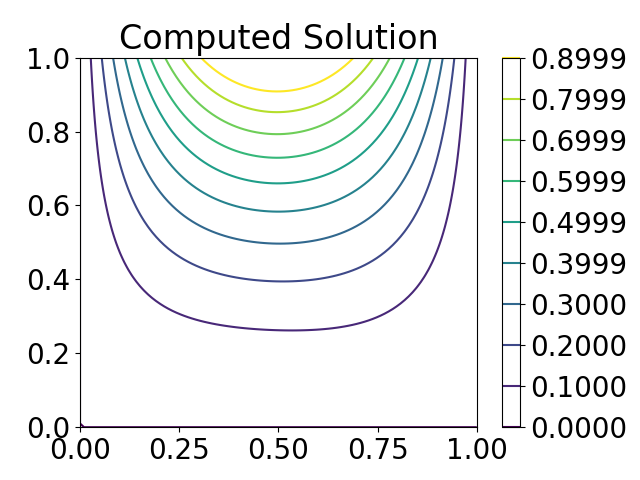
\includegraphics[scale=.5]{hw9 sol}
	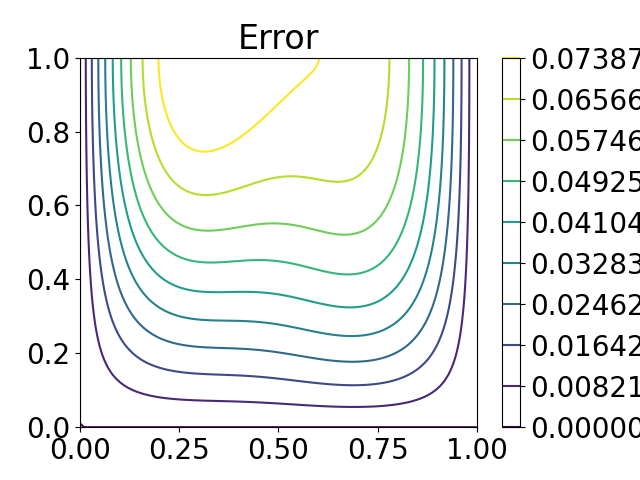
\includegraphics[scale=.5]{hw9 error}
\end{center}
Below is a graph of loss vs iteration number.
\begin{center}
	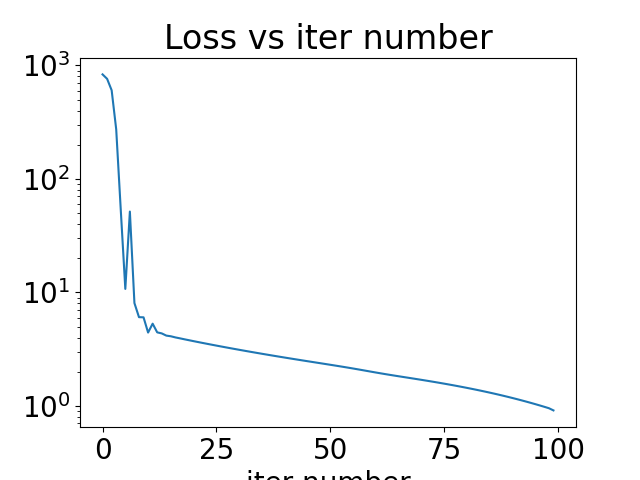
\includegraphics[scale=.3]{hw9 loss}
\end{center}



\item Using separation of variables, write
$$u(x,t) = X(x)T(t)$$
Plug into the PDE.
$$X(x)T'(t) = X''(x)T(t)
\imp \frac{T'(t)}{T(t)} = \frac{X''(x)}{X(x)} = -\lambda
\imp X''+\lambda X=0,~T'+\lambda T=0$$
The eigenvalue problem for $X$,
$$X''+\lambda X = 0, ~X(0) = X'(\pi) = 0$$
has eigenvalues and eigenfunctions
$$\lambda_n = (n+1/2)^2,
~X_n(x) = \sin[(n+1/2)x],
~n\ge 0$$
Solving the ODE for $T$,
$$\quad T'+\lambda_n T=0
\imp T(t) = e^{-\lambda n}t$$
Thus the solution to the BVP is, for some coefficients $a_n$,
$$u(x,t) = \sum_{n\ge0}a_ne^{-(n+1/2)^2t}\sin[(n+1/2)x]$$
Applying the IC,
$$x = u\eval_{t=0} = \sum_{n\ge0}a_n\sin[(n+1/2)x]$$
Fix $m\ge0$, multiply each side by $X_m(x)$, and integrate on $[0,\pi]$. Using the fact $\int_0^\pi X_n(x)X_m(x)dx=\frac\pi2\delta_{nm}$, the RHS becomes
$$\int_0^\pi \sum_{n\ge0}a_nX_n(x)X_m(x)dx = \sum_{n\ge0}a_n\int_0^\pi X_n(x)X_m(x)dx
= \sum_{n\ge0}a_n\frac\pi2 \delta_{nm}
= a_m\frac\pi2$$
Integrating by parts, the LHS becomes
$$\int_0^\pi x\sin[(m+1/2)x]dx = \sbr{-\frac{1}{m+1/2}x\cos[(m+1/2)x] + \frac{1}{(m+1/2)^2}\sin[(m+1/2)x]}\eval_0^\pi$$
$$= -0 + 0 + \frac{1}{(m+1/2)^2}(-1)^{m} - 0
= \frac{(-1)^{m}}{(m+1/2)^2}$$
Thus
$$a_m\frac\pi2 = \frac{(-1)^{m}}{(m+1/2)^2}
\imp a_m = \frac{2(-1)^{m+1}}{\pi(m+1/2)^2}$$

Code:
\url{https://github.com/RokettoJanpu/scientific-computing-2-redux/blob/main/hw9%20q2.ipynb}

\begin{center}
	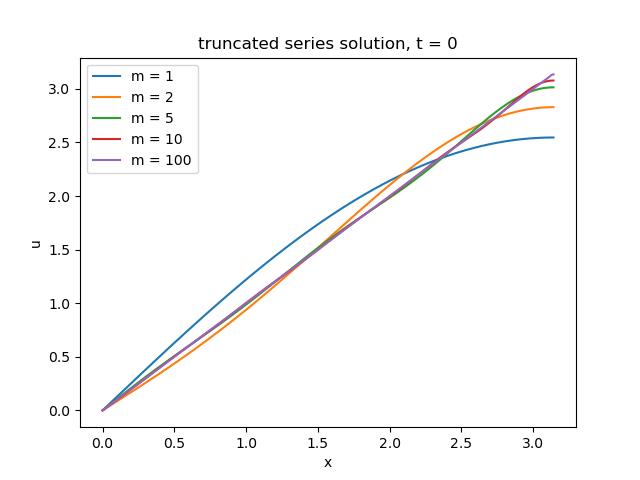
\includegraphics[scale=.4]{hw9 q2 t=0}
	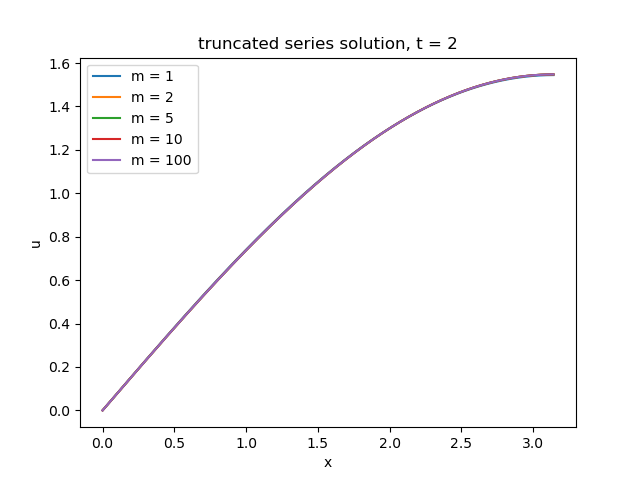
\includegraphics[scale=.4]{hw9 q2 t=2}
\end{center}

In the same ipynb file, we find that the maximum value of $|u(x,0)-x|$ for $m = 100$ is about $6.37\times10^{-3}$.



\end{enumerate}


	
\end{document}